\chapter{Equilibrium}
\index{Equilibrium%
@\emph{Equilibrium}}%


%\pagestyle{empty}

This chapter defines the model equilibria.  We define both the stationary-steady-state equilibrium as well as the stationary non-steady state equilibrium.  Our solution method, described in the next chapter, uses both of these concepts.

 \section{Market clearing and stationary equilibrium}\label{SecMCEqlbm}

    Labor market clearing requires that aggregate demand for effective labor units $EL_t$  equal the sum of individual efficiency units of labor supplied, $e_{j,s}n_{j,s,t}$. Asset market clearing requires that aggregate asset holdings equal the total about of debt and equity asset outstanding. Aggregate consumption $C_t$ is defined as the sum of all individual consumption, and aggregate investment is defined by the resource constant, $Y = C + I$. In particular, we have market clearing in the labor, asset, and goods markets: 
    \begin{align}
     & \sum_{m=1}^{M} EL_{m,c,t} +  \sum_{m=1}^{M} EL_{m,nc,t} + EL^{G}_{t} = \sum_{s=E+1}^{E+S}\sum_{j=1}^{J} \omega_{s,t}\lambda_j e_{j,s}n_{j,s,t} \quad \forall t \label{EqMktClrLab} \\
      & D_{t} +  \sum_{m=1}^{M} B_{m,c,t} +  \sum_{m=1}^{M} B_{m,nc,t} + \sum_{m=1}^{M} V_{m,c,t} +  \sum_{m=1}^{M} V_{m,nc,t}  = \sum_{s=E+2}^{E+S+1}\sum_{j=1}^{J}\omega_{s-1,t-1}\lambda_j b_{j,s,t}  \quad \forall t \label{EqMktClrAsset} \\
   &   \sum_{m=1}^{M} X_{m,c,t} +  \sum_{m=1}^{M} X_{m,nc,t}   = \sum_{s=E+1}^{E+S}\sum_{j=1}^{J}\sum_{i=1}^{I}\omega_{s,t}\lambda_j c_{i,j,s,t} + \sum_{m=1}^{M} I_{m,c,t} +  \sum_{m=1}^{M} I_{m,nc,t} + I^{G}_{t}  \quad\forall t \\
 \label{EqMktClrGoods}
    \end{align}

    The usual definition of equilibrium would be allocations and prices such that households optimize \eqref{Eqcfoc}, \eqref{Eqnfoc}, and \eqref{Eqbfoc}, firms optimize \eqref{eqn:foc_i} and \eqref{eqn:foc_l}, and markets clear \eqref{EqMktClrLab}, \eqref{EqMktClrAsset}, and \eqref{EqMktClrGoods}. However, the variables in these characterizing equations are potentially not stationary due to the possible growth rate in the total population $g_{n,t}$ each period coming from the cohort growth rates in \eqref{EqPopLawofmotion} and from the deterministic growth rate of labor augmenting technological change $g_y$ in \eqref{eqn:prod_fun}.

    \begin{table}[htbp] \centering \captionsetup{width=3.3in}
    \caption{\label{TabStatVars}\textbf{Stationary variable definitions}}
      \begin{threeparttable}
      \begin{tabular}{>{\small}c >{\small}c >{\small}c |>{\small}c}
        \hline\hline
        \multicolumn{3}{c}{Sources of growth} & Not \\
        & & & \\[-4mm]
        $e^{g_y t}$ & $\tilde{N}_t$ & $e^{g_y t}\tilde{N}_t$ & growing\tnote{a} \\
        \hline
        & & \\[-4mm]
        $\hat{c}_{j,s,t}\equiv\frac{\tilde{c}_{j,s,t}}{e^{g_y t}}$ & $\hat{\omega}_{s,t}\equiv\frac{\omega_{s,t}}{\tilde{N}_t}$ & $\hat{X}_t\equiv\frac{X_t}{e^{g_y t}\tilde{N}_t}$ & $n_{j,s,t}$ \\[2mm]
        $\hat{b}_{j,s,t}\equiv\frac{b_{j,s,t}}{e^{g_y t}}$ & $\hat{EL}_t\equiv\frac{EL_t}{\tilde{N}_t}$ & $\hat{K}_t\equiv\frac{K_t}{e^{g_y t}\tilde{N}_t}$ & $r_t$ \\[2mm]
        $\hat{w}_t\equiv\frac{w_t}{e^{g_y t}}$ &  & $\hat{BQ}_{j,t}\equiv\frac{BQ_{j,t}}{e^{g_y t}\tilde{N}_t}$ &  \\[2mm]
        $\hat{y}_{j,s,t}\equiv \frac{y_{j,s,t}}{e^{g_y t}}$ &  & $\hat{I}_{t}\equiv \frac{I_{t}}{e^{g_{y} t}\tilde{N}_t}$ &  \\[2mm]
        $\hat{T}_{j,s,t}\equiv\frac{T_{j,s,t}}{e^{g_y t}}$ &  &  &  \\[2mm]
        $\hat{p}_{s,t}\equiv\frac{\tilde{p}_{s,t}}{e^{g_y t}}$ &  &  &  \\[2mm]
        $\hat{p}_{i,t}\equiv\frac{p_{i,t}}{e^{g_y t}}$ &  &  &  \\[2mm]
        \hline\hline
      \end{tabular}
      \begin{tablenotes}
        \scriptsize{\item[a]The interest rate $r_t$ is already stationary because $X_t$ and $K_t$ grow at the same rate. Individual labor supply, $n_{j,s,t}$, is stationary.}
      \end{tablenotes}
      \end{threeparttable}
    \end{table}

%% Might need more variables in the above

    Table \ref{TabStatVars} characterizes the stationary versions of the variables of the model in terms of the variables that grow due to labor augmenting technological change, population growth, both, or none. With the definitions in Table \ref{TabStatVars}, it can be shown that the equilibrium characterizing equations can be written in stationary form in the following way. The static and intertemporal Euler equations from the individual's optimization problem corresponding to \\eqref{Eqcfoc}, \eqref{Eqnfoc}, and \eqref{Eqbfoc} are the following:
    
    NEED TO UPDATE EQUATIONS...need individual and firm conditions, stationarized...

%    \begin{equation}\label{EqEulerLabStat}
%      \begin{split}
%        &(\hat{c}_{j,s,t})^{-\sigma}\Biggl(\hat{w}_t e_{j,s} - \frac{\partial\hat{T}_{j,s,t}}{\partial n_{j,s,t}}\Biggr) = \chi^n_{s}\biggl(\frac{b}{\tilde{l}}\biggr)\biggl(\frac{n_{j,s,t}}{\tilde{l}}\biggr)^{v-1}\Biggl[1 - \biggl(\frac{n_{j,s,t}}{\tilde{l}}\biggr)\Biggr]^{\frac{1-v}{v}} \\
%        &\qquad\qquad\qquad\qquad\qquad\qquad\qquad\qquad\forall j,t, \quad\text{and}\quad E+1\leq s\leq E+S \\
%        &\qquad\text{where}\quad \hat{c}_{j,s,t} = \left(1 + r_t\right)\hat{b}_{j,s,t} + \hat{w}_t e_{j,s}n_{j,s,t} + \frac{\hat{BQ}_{j,t}}{\lambda_j} - e^{g_y}\hat{b}_{j,s+1,t+1} - \hat{T}_{j,s,t} \\
%        &\qquad\text{and}\quad \frac{\partial \hat{T}_{j,s,t}}{\partial n_{j,s,t}} = \hat{w}_t e_{j,s}\biggl[\tau^I\bigl(F\hat{a}_{j,s,t}\bigr) + \frac{F\hat{a}_{j,s,t}CD\bigl[2A(F\hat{a}_{j,s,t})+B\bigr]}{\bigl[A(F\hat{a}_{j,s,t})^2+B(F \hat{a}_{j,s,t})+C\bigr]^2} + \tau^P\Biggr] \\
%        &\qquad\text{and}\quad \hat{b}_{j,E+1,t} = 0 \quad\forall j,t
%      \end{split}
%    \end{equation}
%
%    \begin{equation}\label{EqEulerSavStat}
%      \begin{split}
%        &(\hat{c}_{j,s,t})^{-\sigma} = ... \\
%        &e^{-g_y\sigma}\Biggl(\rho_s\chi^b \bigl(\hat{b}_{j,s+1,t+1}\bigr)^{-\sigma} + \beta(1-\rho_s)(\hat{c}_{j,s+1,t+1})^{-\sigma}\Biggl[(1 + r_{t+1}) - \frac{\partial T_{j,s+1,t+1}}{\partial b_{j,s+1,t+1}}\Biggr]\Biggr) \\
%        &\qquad\qquad\qquad\qquad\qquad\qquad\qquad\qquad\forall j,t,\quad\text{and}\quad E+1\leq s \leq E+S-1 \\
%        &\qquad\text{where}\quad \frac{\partial T_{j,s+1,t+1}}{\partial b_{j,s+1,t+1}} = ...\\
%        &\qquad\qquad r_{t+1}\Biggl(\tau^I(F\hat{a}_{j,s+1,t+1}) + \frac{F\hat{a}_{j,s+1,t+1}CD\left[2A(F\hat{a}_{j,s+1,t+1}) + B\right]}{\left[A(F\hat{a}_{j,s+1,t+1})^2 + B(F\hat{a}_{j,s+1,t+1}) + C\right]^2}\Biggr) ... \\
%        &\qquad\qquad \tau^W(\hat{b}_{j,s+1,t+1}) + \frac{\hat{b}_{j,s+1,t+1}PHM}{\left(H\hat{b}_{j,s+1,t+1} + M\right)^2}
%      \end{split}
%    \end{equation}
%
%    \begin{equation}\label{EqEulerSavEpSstat}
%      (\hat{c}_{j,E+S,t})^{-\sigma} = \chi^b e^{-g_y\sigma}(\hat{b}_{j,E+S+1,t+1})^{-\sigma} \quad\forall j,t
%    \end{equation}
%
%    The stationary firm first order conditions for optimal labor and capital demand corresponding to \eqref{EqFOCwage} and \eqref{EqFOCrate} are the following.
%    \begin{equation}\label{EqFOCwageStat}
%       \hat{w}_t = (1-\alpha)\frac{\hat{Y}_t}{\hat{L}_t} \quad \forall t
%    \end{equation}
%    \begin{equation}\tag{\ref{EqFOCrate}}
%       r_t = \alpha\frac{\hat{Y}_t}{\hat{K}_t} - \delta = \alpha\frac{Y_t}{K_t} - \delta \quad \forall t
%    \end{equation}
%    And the two stationary market clearing conditions corresponding to \eqref{EqMktClrLab} and \eqref{EqMktClrCap}---with the goods market clearing by Walras' Law---are the following.
%    \begin{align}
%      \hat{L}_t &= \sum_{s=E+1}^{E+S}\sum_{j=1}^{J} \hat{\omega}_{s,t}\lambda_j e_{j,s}n_{j,s,t} \quad \forall t \label{EqMktClrLabStat} \\
%      \hat{K}_t &= \frac{1}{1 + \tilde{g}_{n,t}}\left(\sum_{s=E+2}^{E+S+1}\sum_{j=1}^{J}\hat{\omega}_{s-1,t-1}\lambda_j \hat{b}_{j,s,t}\right) \quad \forall t \label{EqMktClrCapStat}
%    \end{align}
%    where $\tilde{g}_{n,t}$ is the growth rate in the working age population between periods $t-1$ and $t$ described in \eqref{EqPopWkGrowth}.

    We can now define the stationary steady-state equilibrium for this economy in the following way.

   \ \\
   
    \hrule
    \begin{definition}[\textbf{Stationary steady-state equilibrium}]\label{DefEquilSS}
      A non-autarkic stationary steady-state equilibrium in the overlapping generations model with $S$-period lived agents and heterogeneous ability $e_{j,s}$ is defined as constant allocations $n_{j,s,t}=\bar{n}_{j,s}$ and $\hat{b}_{j,s+1,t+1}=\bar{b}_{j,s+1}$ and constant prices $\hat{w}_t=\bar{w}$ and $r_t=\bar{r}$ for all $j$, $s$, and $t$ such that the following conditions hold:
       \begin{enumerate}
          \item households optimize according to \eqref{EqEulerLabStat}, \eqref{EqEulerSavStat}, and \eqref{EqEulerSavEpSstat},
          \item firms optimize according to \eqref{EqFOCwageStat} and \eqref{EqFOCrate},
          \item markets clear according to\eqref{EqMktClrLab}, \eqref{EqMktClrAsset}, and \eqref{EqMktClrGoods}, and
          \item the population has reached its stationary steady state distribution $\bar{\omega}_s$ for all ages $s$, characterized in Chapter \ref{AppPopGrowth}.
       \end{enumerate}
    \end{definition}
    \hrule

\ \\

    The steady-state equilibrium is characterized by the system of $2JS+4M+...$ equations and $2JS+4M+...$ unknowns $\bar{n}_{j,s}$, $\bar{b}_{j,s+1}$, $EL_{m,c,t}$, $I_{m,c,t}$,... . Chapter \ref{chap:model_soln} details how to solve for the steady-state equilibrium.

%    \begin{table}[htbp] \centering \captionsetup{width=4.7in}
%    \caption{\label{TabExogVars}\textbf{List of exogenous variables and baseline calibration values}}
%      \begin{threeparttable}
%      \begin{tabular}{>{\footnotesize}c |>{\footnotesize}l |>{\footnotesize}c}
%        \hline\hline
%        Symbol & \quad\quad\quad\quad Description & Value \\
%        \hline
%        $\bm{\hat{\Gamma}}_1$ & Initial distribution of savings & $\bm{\bar{\Gamma}}$ \\
%        $N_0$ & Initial population & 1 \\
%        $\{\omega_{s,0}\}_{s=1}^S$ & Initial population by age & (see App. \ref{AppPopGrowth}) \\
%        $\{f_s\}_{s=1}^S$ & Fertility rates by age & (see App. \ref{AppPopGrowth}) \\
%        $\{i_s\}_{s=1}^S$ & Immigration rates by age & (see App. \ref{AppPopGrowth}) \\
%        $\{\rho_s\}_{s=1}^S$ & Mortality rates by age & (see App. \ref{AppPopGrowth}) \\
%        $\{e_{j,s}\}_{j,s=1}^{J,S}$ & Deterministic ability process & (see App. \ref{AppAbilCalib}) \\
%        $\{\lambda_j\}_{j=1}^J$ & Ability type bin percentages & (see App. \ref{AppAbilCalib}) \\
%        $J$ & Number of ability types & 7 \\
%        $S$ & Maximum periods in economically active & 80 \\[-2mm]
%        &\quad household life & \\
%        $E$ & Number of periods of youth economically & $\text{round}\left(\frac{S}{4}\right)$ \\[-2mm]
%        & \quad outside the model & \\
%        $R$ & Retirement age (period) & $\text{round}\left(\frac{9}{16}S\right)$ \\
%        \hline
%        $\tilde{l}$ & Maximum hours of labor supply & 1 \\
%        $\beta$ & Discount factor & $(0.96)^\frac{80}{S}$ \\
%        $\sigma$ & Coefficient of constant relative risk aversion & 3 \\
%        $b$ & Scale parameter in utility of leisure & (see App. \ref{AppEllipseUtil}) \\
%        $\upsilon$ & Shape parameter in utility of leisure & (see App. \ref{AppEllipseUtil}) \\
%        $k$ & constant parameter in utility of leisure & (see App. \ref{AppEllipseUtil}) \\
%        $\chi^n_s$ & Disutility of labor level parameter & (see App. \ref{AppChinsChib}) \\
%        $\chi^b$ & Utility of bequests level parameter & (see App. \ref{AppChinsChib}) \\
%        \hline
%        $Z$ & Level parameter in production function & 1 \\
%        $\alpha$ & Capital share of income & 0.35 \\
%        $\delta$ & Capital depreciation rate & $1-(1-0.05)^\frac{80}{S}$ \\
%        $g_y$ & Growth rate of labor augmenting & $(1+0.03)^\frac{80}{S}-1$ \\[-2mm]
%        & \quad technological progress & \\
%        \hline
%        $A$ & Coefficient on squared term in $\tau^I(\cdot)$ & (see App. \ref{AppIncTaxRate}) \\
%        $B$ & Coefficient on linear term in $\tau^I(\cdot)$ & (see App. \ref{AppIncTaxRate}) \\
%        $C$ & Constant coefficient in $\tau^I(\cdot)$ & (see App. \ref{AppIncTaxRate}) \\
%        $D$ & Level parameter for $\tau^I(\cdot)$ & (see App. \ref{AppIncTaxRate}) \\
%        $F$ & Income factor for $\tau^I(\cdot)$ & (see App. \ref{AppIncTaxRate}) \\
%        $\tau^P$ & Payroll tax rate & 0.15 \\
%        $\{\theta^j\}_{j=1}^J$ & Replacement rate by average income & (see App. \ref{AppReplRate}) \\
%        $\tau^{BQ}$ & Bequest (estate) tax rate & 0 \\
%        $P$ & Level parameter for $\tau^W(\cdot)$ & 0 \\
%        $H$ & Coefficient on linear term in $\tau^W(\cdot)$ & 0 \\
%        $M$ & Constant coefficient in $\tau^W(\cdot)$ & 0 \\
%        \hline
%        $T$ & Number of periods to steady state & 160 \\
%        $\nu$ & Dampening parameter for TPI & 0.2 \\
%        \hline\hline
%      \end{tabular}
%      % \begin{tablenotes}
%      %   \scriptsize{\item[]Note: Maybe put sources here.}
%      % \end{tablenotes}
%      \end{threeparttable}
%    \end{table}
%
%    \begin{figure}[htb]\centering \captionsetup{width=4.0in}
%      \caption{\label{FigLogSavSS}\textbf{Stationary steady-state distribution of savings $\log(\bar{\bm{\Gamma}})$ for $S=80$ and $J=7$}}
%      \fbox{\resizebox{4.0in}{3.0in}{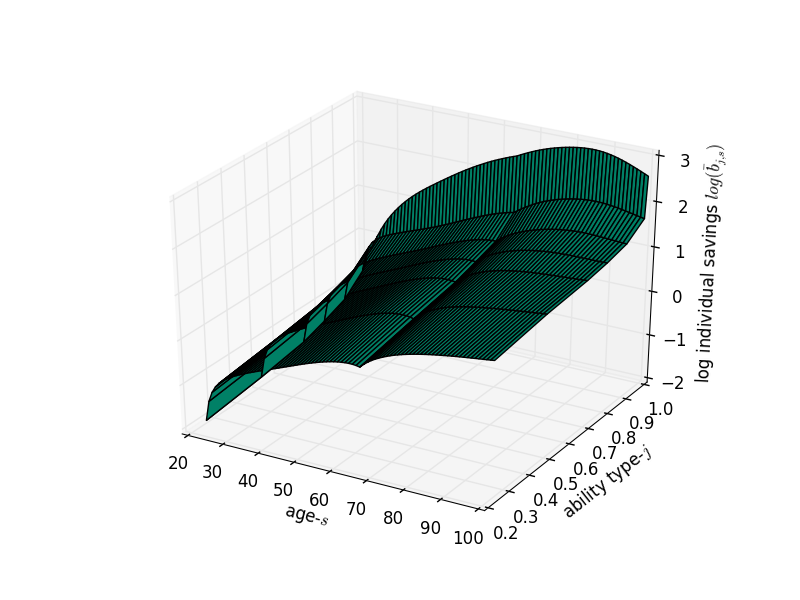
\includegraphics{images/SavSS_log.png}}}
%    \end{figure}
%
%    \begin{figure}[htb]\centering \captionsetup{width=4.0in}
%      \caption{\label{FigLabSS}\textbf{Stationary steady-state distribution of individual labor supply $\bar{n}_{j,s}$ for $S=80$ and $J=7$}}
%      \fbox{\resizebox{4.0in}{3.0in}{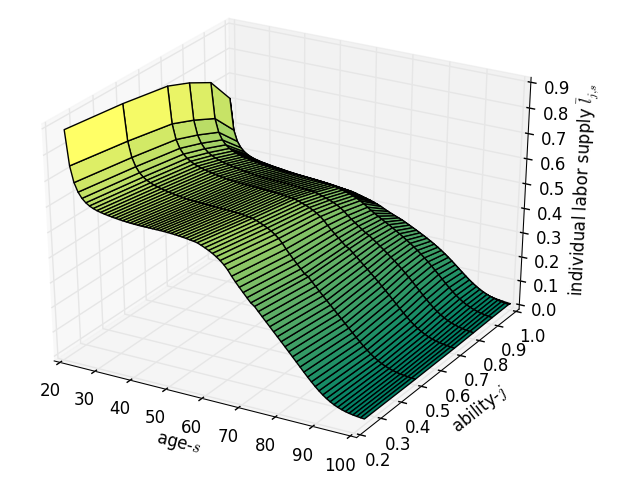
\includegraphics{images/LabSS.png}}}
%    \end{figure}
%
%    \begin{figure}[htb]\centering \captionsetup{width=4.0in}
%      \caption{\label{FigLogConsSS}\textbf{Stationary steady-state distribution of consumption $\bar{c}_{j,s}$ for $S=80$ and $J=7$}}
%      \fbox{\resizebox{4.0in}{3.0in}{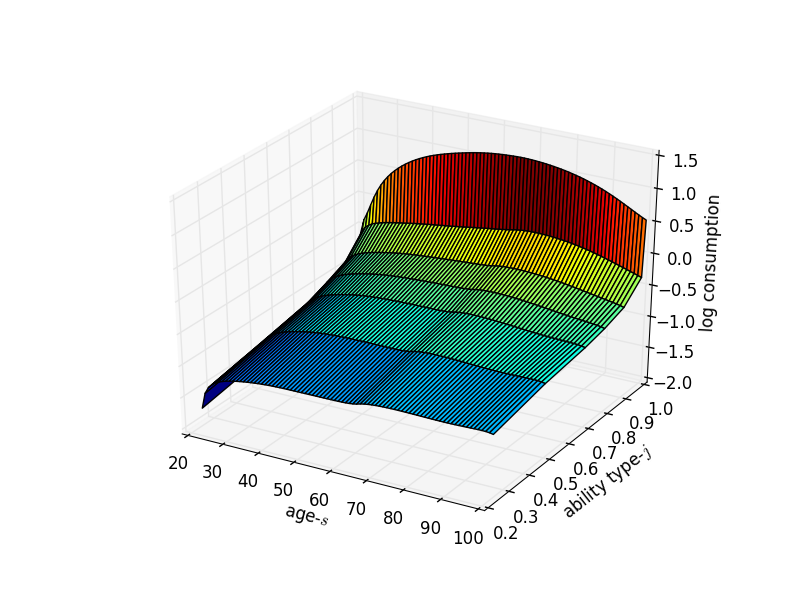
\includegraphics{images/ConsSS_log.png}}}
%    \end{figure}
%
%    Figure \ref{FigLogSavSS} shows the stationary steady-state distribution of individual savings $\bar{b}_{j,s}$ in logarithms, Figure \ref{FigLabSS} shows the stationary steady-state distribution of individual labor supply $\bar{n}_{j,s}$, and Figure \ref{FigLogConsSS} shows the steady-state distribution of consumption $\bar{c}_{j,s}$ in logarithms for a particular calibration of the model described in Table \ref{TabExogVars}. Notice from Figure \ref{FigLogConsSS} the hump-shaped pattern of consumption over the life cycle for each ability type, which is consistent with consumption data. Also note from the comparison of the distribution of savings in Figure \ref{FigLogSavSS} in comparison to the distribution of consumption in \ref{FigLogConsSS} that households use savings to smooth out consumption as much as possible, with a sharpe change in savings around retirement $s=R$ and only a small smooth lump in consumption at that age.

    The definition of the stationary non-steady-state equilibrium is similar to Definition \ref{DefEquilSS}, with the stationary steady-state equilibrium definition being a special case of the stationary non-steady-state equilibrium.

\ \\ 
WHAT FOLLOWS NEEDS UPDATING TO INCLUDE RICHER FIRM AND GOV'T, BUT IS HELPFUL IN SEEING THAT NON-SS EQ'M WILL LOOK LIKE...

\ \\

    \hrule
    \begin{definition}[\textbf{Stationary non-steady-state equilibrium}]\label{DefEquilNonSS}
      A non-autarkic stationary non-steady-state equilibrium in the overlapping generations model with $S$-period lived agents and heterogeneous ability $e_{j,s}$ is defined as allocations $n_{j,s,t}$ and $\hat{b}_{j,s+1,t+1}$ and prices $\hat{w}_t$ and $r_t$ for all $j$, $s$, and $t$ such that the following conditions hold:
       \begin{enumerate}
          \item households have symmetric beliefs $\Omega(\cdot)$ about the evolution of the distribution of savings, and those beliefs about the future distribution of savings equal the realized outcome (rational expectations),
            \begin{equation*}
              \bm{\hat{\Gamma}}_{t+u} = \bm{\hat{\Gamma}}^e_{t+u} = \Omega^u\left( \bm{\hat{\Gamma}}_t\right) \quad\forall t, \quad u\geq 1
            \end{equation*}
          \item households optimize according to \eqref{EqEulerLabStat}, \eqref{EqEulerSavStat}, and \eqref{EqEulerSavEpSstat}
          \item firms optimize according to \eqref{EqFOCwageStat} and \eqref{EqFOCrate}, and
          \item markets clear according to \eqref{EqMktClrLabStat} and \eqref{EqMktClrCapStat}.
       \end{enumerate}
    \end{definition}
    \hrule
   
   \ \\
   
    \noindent Taken together, the household labor-leisure and intended bequest decisions in the last period of life show that the optimal labor supply and optimal intended bequests for age $s=E+S$ are each functions of individual holdings of savings, total bequests received, and the prices in that period $n_{j,E+S,t}=\phi\bigl(\hat{b}_{j,E+S,t},\hat{BQ}_{j,t},\hat{w}_t,r_t\bigr)$ and $\hat{b}_{j,E+S+1,t+1}=\psi\bigl(\hat{b}_{j,E+S,t},\hat{BQ}_{j,t},\hat{w}_t,r_t\bigr)$. These two decisions are characterized by final-age version of the static labor supply Euler equation \eqref{EqEulerLabStat} and the static intended bequests Euler equation \eqref{EqEulerSavEpSstat}. Households in their second-to-last period of life in period $t$ have four decisions to make. They must choose how much to work this period $n_{j,E+S-1,t}$ and next period $n_{j,E+S,t+1}$, how much to save this period for next period $\hat{b}_{j,E+S,t+1}$, and how much to bequeath next period $\hat{b}_{j,E+S+1,t+2}$. The optimal responses for this individual are characterized by the $s=E+S-1$ and $s=E+S$ versions of the static Euler equations \eqref{EqEulerLabStat}, the $s=E+S-1$ version of the intertemporal Euler equation \eqref{EqEulerSavStat}, and the $s=E+S$ static bequest Euler equation \eqref{EqEulerSavEpSstat}, respectively.

    Optimal savings in the second-to-last period of life $s=E+S-1$ is a function of the current savings as well as the total bequests received and prices in the current period and in the next period $\hat{b}_{j,E+S,t+1} = \psi\bigl(\hat{b}_{j,E+S-1,t},\hat{BQ}_{j,t},\hat{w}_t,r_t,\hat{BQ}_{j,t+1},\hat{w}_{t+1},r_{t+1}|\Omega\bigr)$ given beliefs $\Omega$. As before, the optimal labor supply at age $s=E+S$ is a function of the next period's savings, bequests received, and prices $n_{j,E+S,t+1}=\phi\bigl(\hat{b}_{j,E+S,t+1},\hat{BQ}_{j,t+1},\hat{w}_{t+1},r_{t+1}\bigr)$. But the optimal labor supply at age $s=E+S-1$ is a function of the current savings, current bequests received, and the current prices as well as the future bequests received and future prices because of the dependence on the savings decision in that same period $n_{j,E+S-1,t}=\phi\bigl(\hat{b}_{j,E+S-1,t},\hat{BQ}_{j,t},\hat{w}_t,r_t,\hat{BQ}_{j,t+1},\hat{w}_{t+1},r_{t+1}|\Omega\bigr)$ given beliefs $\Omega$. By induction, we can show that the optimal labor supply, savings, and intended bequests functions for any individual with ability $j$, age $s$, and in period $t$ is a function of current holdings of savings and the lifetime path of total bequests received and prices given beliefs $\Omega$.
    \begin{align}
      n_{j,s,t} &= \phi\Bigl(\hat{b}_{j,s,t},\bigl(\hat{BQ}_{j,v},\hat{w}_v,r_v\bigr)_{v=t}^{t+S-s}|\Omega\Bigr) \quad\forall j,s,t \label{EqLabPolFuncGen} \\
      \hat{b}_{j,s+1,t+1} &= \psi\Bigl(\hat{b}_{j,s,t},\bigl(\hat{BQ}_{j,v},\hat{w}_v,r_v\bigr)_{v=t}^{t+S-s}|\Omega\Bigr) \quad\forall j,t \quad\text{and}\quad E+1\leq s\leq E+S \label{EqSavPolFuncGen}
    \end{align}

    If one knows the current distribution of households savings and intended bequests $\bm{\hat{\Gamma}}_t$ and has a beliefs function that predicts the law of motion over time for $\bm{\hat{\Gamma}}_t$, then one can predict time series for total bequests received $\hat{BQ}_{j,t}$, real wages $\hat{w}_t$ and real interest rates $r_t$ necessary for solving each household's optimal decisions. Characteristic (i) in equilibrium definition \ref{DefEquilNonSS} that individuals be able to forecast prices with perfect foresight over their lifetimes implies that each individual has correct information and beliefs about all the other individuals optimization problems and information. It also implies that the equilibrium allocations and prices are really just functions of the entire distribution of savings at a particular period, as well as a law of motion for that distribution of savings.

    In equilibrium, the steady-state household labor supplies $\bar{n}_{j,s}$ for all $j$ and $s$, the steady-state savings $\bar{b}_{j,E+S+1}$, the steady-state real wage $\bar{w}$, and the steady-state real rental rate $\bar{r}$ are simply functions of the steady-state distribution of savings $\bar{\Gamma}$. This is clear from the steady-state version of the capital market clearing condition \eqref{EqMktClrCapStat} and the fact that aggregate labor supply is a function of the sum of exogenous efficiency units of labor in the labor market clearing condition \eqref{EqMktClrLabStat}. And the two firm first order conditions for the real wage $\hat{w}_t$ \eqref{EqFOCwageStat} and real rental rate $r_t$ \eqref{EqFOCrate} are only functions of the stationary aggregate capital stock $\hat{K}_t$ and aggregate labor $\hat{L}_t$.

    \begin{figure}[htb]\centering \captionsetup{width=4.0in}
      \caption{\label{FigKpathTPI}\textbf{Equilibrium time path of $K_t$ for $S=80$ and $J=7$}}
      \fbox{\resizebox{4.0in}{3.0in}{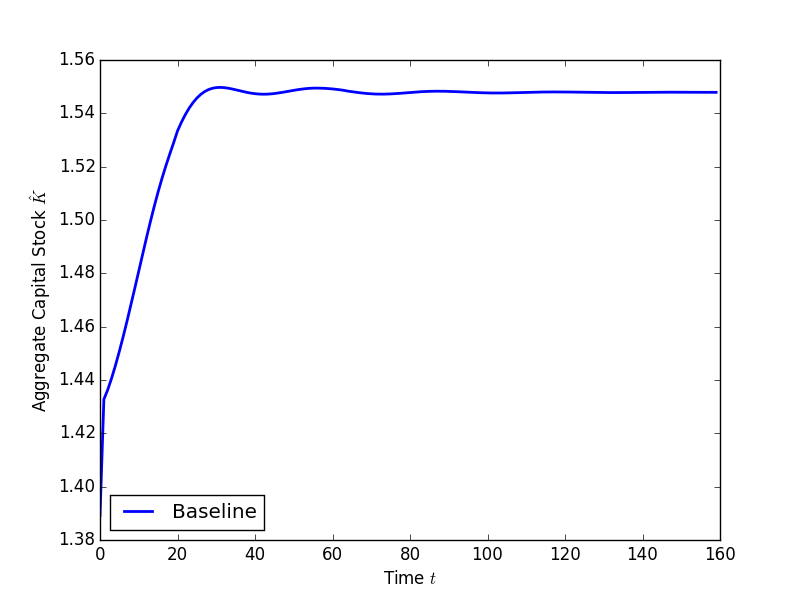
\includegraphics{images/KpathTPI.png}}}
    \end{figure}

    \begin{figure}[htb]\centering \captionsetup{width=4.0in}
      \caption{\label{FigLpathTPI}\textbf{Equilibrium time path of $L_t$ for $S=80$ and $J=7$}}
      \fbox{\resizebox{4.0in}{3.0in}{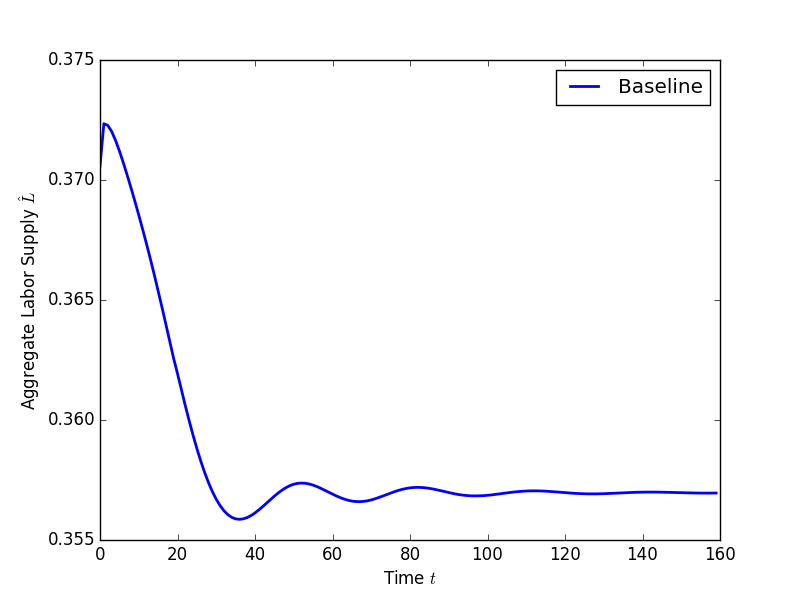
\includegraphics{images/LpathTPI.png}}}
    \end{figure}

